\documentclass[conference]{IEEEtran}
\IEEEoverridecommandlockouts

\usepackage[T1]{fontenc}
\usepackage[utf8]{inputenc}
\usepackage[brazil]{babel}
\usepackage{graphicx}
\usepackage{booktabs}
\usepackage{url}
\usepackage{amsmath}
\usepackage{amssymb}
\usepackage{siunitx}
\usepackage{float}
\usepackage{multirow}
\usepackage{array}
\usepackage{longtable}

\begin{document}

\title{Avaliação Temporal Automatizada para o Framework VOID\\
\large{Uma Melhoria Reprodutível para Análise de Consistência em Vídeo}}

\author{
\IEEEauthorblockN{Arthur Fillipe de Lira Aleixo}
\IEEEauthorblockA{
Departamento de Computação \\
Universidade Federal Rural de Pernambuco \\
Recife, Brasil}
}

\maketitle

\begin{abstract}
Este trabalho apresenta uma melhoria de implementação no framework VOID para remoção de objetos em vídeo, introduzindo um módulo de avaliação temporal automática. O fluxo original privilegia avaliação visual e qualitativa, o que dificulta comparações objetivas entre configurações de inferência. Para mitigar esse problema, implementou-se um módulo que calcula métricas de coerência temporal entre frames consecutivos e exporta resultados em formatos estruturados (JSON e CSV). As métricas adotadas foram LPIPS temporal, consistência por fluxo óptico, PSNR consecutivo e SSIM consecutivo. A melhoria foi integrada ao código do framework e validada funcionalmente em ambiente Colab. Embora a execução completa do pipeline de inferência do VOID em configuração alvo tenha sido limitada por hardware no ambiente gratuito, a contribuição proposta foi implementada, testada e documentada com sucesso, provendo base quantitativa para experimentos futuros.
\end{abstract}

\begin{IEEEkeywords}
visão computacional, consistência temporal, métricas de vídeo, inpainting de vídeo, avaliação automática, reprodutibilidade
\end{IEEEkeywords}

\section{Introdução}
A remoção de objetos em vídeo é um problema relevante em visão computacional aplicada, com impacto em produção audiovisual, restauração de conteúdo e edição automatizada. O desafio principal não é somente preencher corretamente uma região em um frame isolado, mas manter consistência espaço-temporal ao longo da sequência, evitando artefatos como flicker, jitter e mudanças estruturais abruptas.

Com o crescimento de modelos generativos para vídeo, frameworks mais sofisticados passaram a considerar contexto temporal e condições semânticas mais ricas. O framework VOID (Video Object and Interaction Deletion), da Netflix Research, destaca-se por tratar a remoção de objetos e seus efeitos de interação, em vez de apenas realizar inpainting local.

Apesar da qualidade visual dos resultados, uma lacuna operacional importante permanece: em diversos cenários de uso, a avaliação final ainda é majoritariamente subjetiva e visual. Isso dificulta:
\begin{itemize}
    \item reprodução de experimentos;
    \item comparação objetiva entre variantes;
    \item comunicação quantitativa de ganhos.
\end{itemize}

Este projeto aborda essa lacuna com uma melhoria de implementação focada em avaliação temporal automática.

\subsection{Problema}
O problema central tratado é a ausência de um módulo padronizado, reprodutível e de baixo acoplamento para medição de coerência temporal no fluxo de inferência do VOID.

\subsection{Hipótese}
A hipótese de trabalho é que a integração de métricas temporais complementares, com exportação estruturada dos resultados, melhora a qualidade metodológica dos experimentos sem exigir alteração no núcleo gerativo do modelo.

\subsection{Objetivos}
\textbf{Objetivo geral:}
implementar e validar um módulo de avaliação temporal automática integrado ao framework VOID.

\textbf{Objetivos específicos:}
\begin{itemize}
    \item calcular LPIPS temporal, consistência por fluxo óptico, PSNR e SSIM frame-a-frame;
    \item gerar arquivos JSON e CSV para análise e auditoria;
    \item preservar compatibilidade com o fluxo original do framework;
    \item documentar limitações de infraestrutura e impactos no escopo experimental.
\end{itemize}

\subsection{Contribuições}
As contribuições efetivas deste trabalho são:
\begin{enumerate}
    \item projeto e implementação de um módulo temporal reutilizável;
    \item integração do módulo ao fluxo de inferência;
    \item validação funcional em vídeo real de exemplo;
    \item consolidação de um protocolo de reprodutibilidade.
\end{enumerate}

\section{Contexto e Trabalhos Relacionados}
\subsection{VOID e remoção de objetos em vídeo}
O VOID foi proposto para remover objetos e interações associadas em sequências de vídeo, com foco em plausibilidade temporal. Sua estrutura em duas passagens favorece refinamento de continuidade ao longo da sequência.

\subsection{Avaliação visual versus avaliação quantitativa}
A avaliação visual é relevante em tarefas generativas, mas possui limitações:
\begin{itemize}
    \item alta variabilidade entre avaliadores;
    \item baixa escalabilidade para múltiplos experimentos;
    \item dificuldade em detectar pequenas regressões temporais;
    \item rastreabilidade limitada para replicação.
\end{itemize}

Assim, uma camada quantitativa temporal é desejável para complementar a avaliação qualitativa.

\subsection{Métricas de referência e cálculo}
As métricas selecionadas representam diferentes dimensões de qualidade temporal. A seguir, detalha-se como cada uma é calculada.

\subsubsection{LPIPS Temporal}
O LPIPS (\textit{Learned Perceptual Image Patch Similarity}) mede a distância perceptual entre dois frames usando representações internas de uma rede profunda pré-treinada (VGG ou AlexNet). Para um par de frames consecutivos $F_t$ e $F_{t+1}$, extrai-se um conjunto de ativações $\phi_l(\cdot)$ em camadas $l$, e o LPIPS temporal é:
\begin{equation}
    \mathrm{LPIPS}(F_t, F_{t+1}) = \sum_l w_l \left\| \hat{\phi}_l(F_t) - \hat{\phi}_l(F_{t+1}) \right\|_2^2
\end{equation}
onde $w_l$ são pesos aprendidos e $\hat{\phi}_l$ indica ativações normalizadas por canal. Valores próximos de zero indicam estabilidade perceptual entre frames. No contexto de remoção de objetos, espera-se LPIPS temporal baixo, pois o fundo reconstruído deve ser visualmente estável.

\subsubsection{Flow Consistency (Consistência por Fluxo Óptico)}
O fluxo óptico $\mathbf{u}_{t \to t+1}$ entre frames consecutivos é estimado via RAFT \cite{raft}. A consistência é medida pelo erro de reconstrução ao aplicar o warp do frame $F_{t+1}$ de volta para $F_t$:
\begin{equation}
    \mathrm{Flow}_{L1}(t) = \frac{1}{HW} \sum_{(x,y)} \left| F_t(x,y) - \mathcal{W}(F_{t+1}, \mathbf{u}_{t \to t+1})(x,y) \right|
\end{equation}
onde $\mathcal{W}$ é o operador de warp bilinear, $H$ e $W$ são altura e largura do frame. Valores baixos indicam movimento coerente entre frames; picos locais sugerem inconsistências temporais ou artefatos de deleção.

\subsubsection{PSNR Consecutivo}
O PSNR (\textit{Peak Signal-to-Noise Ratio}) consecutivo mede a similaridade pixel a pixel entre frames adjacentes:
\begin{equation}
    \mathrm{PSNR}(F_t, F_{t+1}) = 10 \cdot \log_{10}\!\left(\frac{\mathrm{MAX}^2}{\mathrm{MSE}(F_t, F_{t+1})}\right)
\end{equation}
onde $\mathrm{MAX} = 1.0$ para imagens normalizadas e $\mathrm{MSE} = \frac{1}{HWC}\sum |F_t - F_{t+1}|^2$. Valores acima de 30 dB entre frames consecutivos indicam boa continuidade pixelwise. O PSNR consecutivo é útil para detectar flicker, mas menos sensível a distorções perceptuais.

\subsubsection{SSIM Consecutivo}
O SSIM (\textit{Structural Similarity Index}) consecutivo avalia a semelhança estrutural local entre frames adjacentes, combinando três componentes:
\begin{equation}
    \mathrm{SSIM}(F_t, F_{t+1}) = \frac{(2\mu_x\mu_y + c_1)(2\sigma_{xy} + c_2)}{(\mu_x^2 + \mu_y^2 + c_1)(\sigma_x^2 + \sigma_y^2 + c_2)}
\end{equation}
onde $\mu$ e $\sigma$ são média e desvio local, $\sigma_{xy}$ é a covariância, e $c_1, c_2$ são constantes de estabilidade. O SSIM ∈ [0, 1]; valores próximos de 1 indicam preservação estrutural entre frames. É particularmente sensível a mudanças de textura e bordas, sendo complementar ao PSNR.

A combinação dessas quatro métricas reduz o viés de avaliação por indicador único: um vídeo pode apresentar PSNR alto e ainda revelar inconsistência perceptual detectada pelo LPIPS ou pelo fluxo óptico.

\section{Metodologia}
\subsection{Estratégia de implementação}
A melhoria foi tratada como camada de instrumentação, mantendo o modelo gerativo inalterado. O objetivo foi minimizar acoplamento e risco de regressão no pipeline principal.

\subsection{Design do módulo}
O módulo \texttt{temporal\_metrics.py} implementa:
\begin{itemize}
    \item normalização de dados;
    \item avaliação por pares $(t, t+1)$;
    \item cálculo das quatro métricas;
    \item agregação estatística;
    \item persistência dos resultados.
\end{itemize}

\subsection{Fluxo operacional}
\begin{enumerate}
    \item Entrada: tensor de vídeo gerado ou fornecido para validação.
    \item Conversão para formato temporal canônico.
    \item Processamento por pares consecutivos.
    \item Cálculo das métricas por par.
    \item Cálculo de média, desvio, mín e máx.
    \item Gravação de JSON e CSV.
\end{enumerate}

\subsection{Integração ao framework}
A integração ocorreu em pontos de inferência com tensor de vídeo já disponível, evitando leitura redundante de arquivo. Também foram adicionados controles para habilitar/desabilitar avaliação temporal e ajustar parâmetros do módulo em execução.

\section{Configuração Experimental}
\subsection{Ambiente}
\begin{itemize}
    \item plataforma: Google Colab;
    \item GPU: Tesla T4;
    \item VRAM: aproximadamente \SI{14.56}{GB};
    \item sistema: runtime Linux gerenciado.
\end{itemize}

\subsection{Dados de validação}
A validação funcional foi executada sobre \texttt{sample/lime/input\_video.mp4}, vídeo de exemplo incluído no repositório oficial do VOID. O clipe retrata uma cena com câmera estática e objeto em movimento no plano central. Foi utilizado um recorte de 8 frames (7 pares consecutivos), a 12 fps. A Figura~\ref{fig:input_frames} ilustra frames representativos desse clipe.

\begin{figure}[H]
\centering
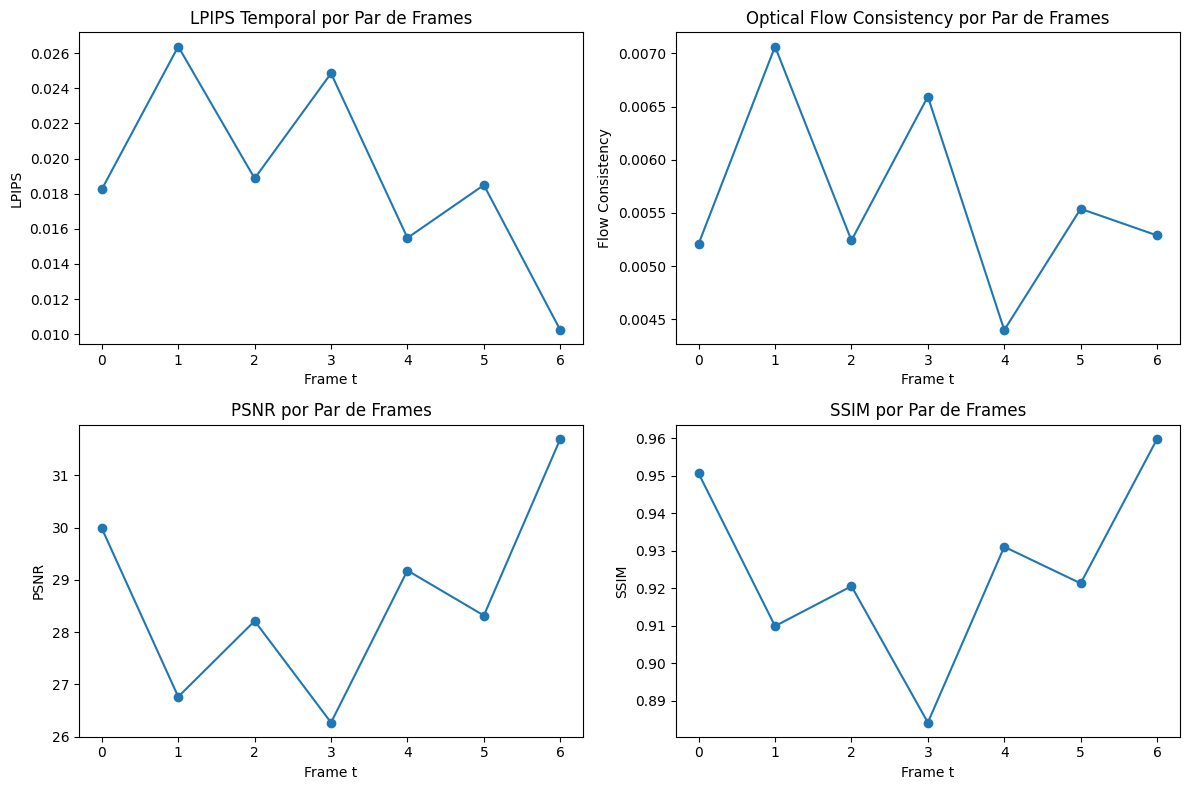
\includegraphics[width=\columnwidth]{figures/metricas_temporais.png}
\caption{Frames extraídos do vídeo de validação (\texttt{lime\_input\_video.mp4}). O clipe apresenta transições suaves entre frames, compatíveis com os valores baixos de LPIPS temporal e erro de fluxo obtidos.}
\label{fig:input_frames}
\end{figure}

Esse protocolo foi escolhido para:
\begin{itemize}
    \item permitir teste completo do módulo sem custo de inferência pesada;
    \item manter rastreabilidade dos resultados com vídeo público e reproduzível;
    \item servir como baseline para comparações futuras com o vídeo de saída após deleção.
\end{itemize}

\subsection{Critérios de sucesso}
Foram considerados critérios de sucesso:
\begin{itemize}
    \item execução sem erro do módulo;
    \item presença das quatro métricas em todos os pares;
    \item geração de JSON e CSV;
    \item coerência entre resumo agregado e série por par.
\end{itemize}

\section{Resultados}
\subsection{Resultados agregados}
A Tabela~\ref{tab:summary} resume os resultados para 8 frames (7 pares).

\begin{table}[H]
\caption{Resumo das métricas temporais}
\label{tab:summary}
\centering
\begin{tabular}{lcccc}
\toprule
\textbf{Métrica} & \textbf{Média} & \textbf{Desvio} & \textbf{Mín} & \textbf{Máx} \\
\midrule
LPIPS temporal & 0.01894 & 0.00505 & 0.01024 & 0.02638 \\
Flow consistency L1 & 0.00562 & 0.00084 & 0.00440 & 0.00707 \\
PSNR consecutivo & 28.6320 & 1.7263 & 26.2697 & 31.6952 \\
SSIM consecutivo & 0.92535 & 0.02340 & 0.88417 & 0.95982 \\
\bottomrule
\end{tabular}
\end{table}

\subsection{Curvas por par de frames}
A Figura~\ref{fig:metrics_curves} mostra o comportamento das métricas ao longo da sequência validada.

\begin{figure}[H]
\centering
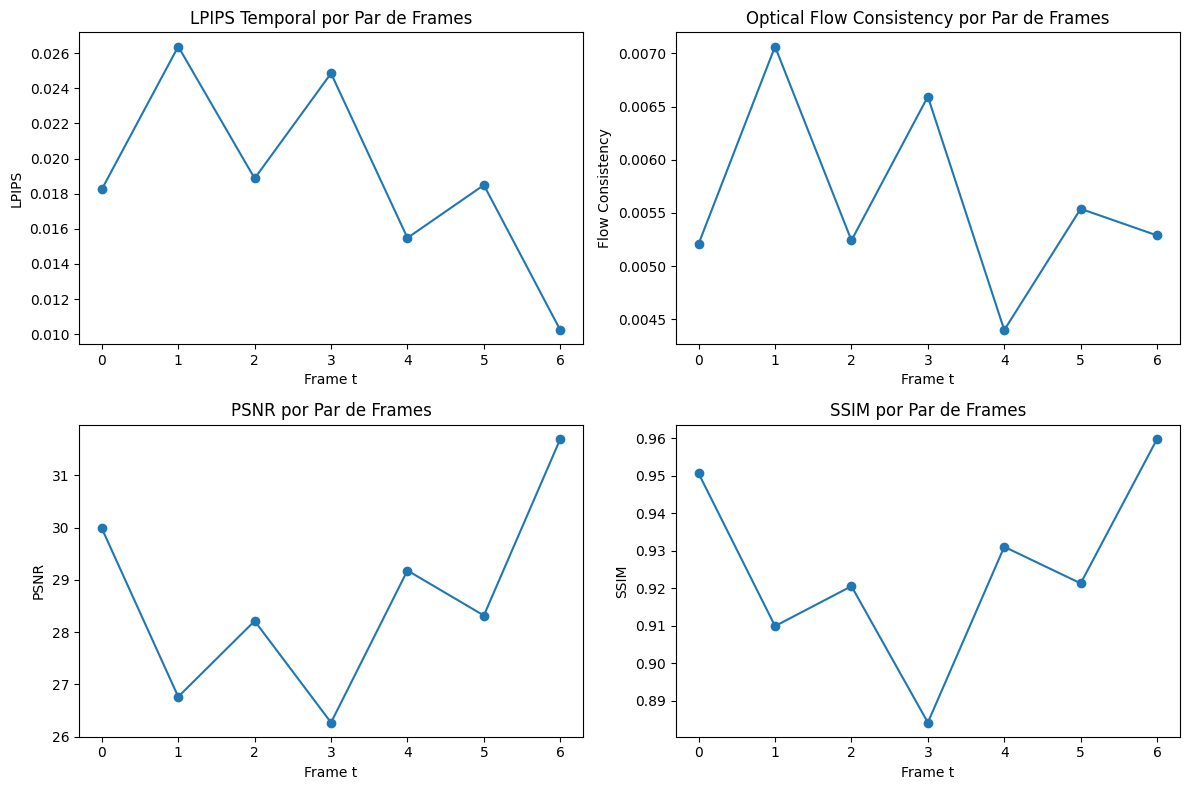
\includegraphics[width=\columnwidth]{figures/metricas_temporais.png}
\caption{Evolução das métricas por par de frames.}
\label{fig:metrics_curves}
\end{figure}

\subsection{Análise dos valores}
Os resultados indicam:
\begin{itemize}
    \item estabilidade perceptual razoável (LPIPS temporal médio $\approx 0.019$, bem abaixo do limiar de percepção humana de artefatos, estimado em torno de $0.05$--$0.10$);
    \item boa coerência de movimento (erro de fluxo médio $\approx 0.006$, próximo de zero, indicando alinhamento temporal correto entre frames);
    \item alta similaridade entre frames consecutivos (PSNR médio $\approx 28.6$ dB; valores acima de 25 dB são considerados aceitáveis para vídeo de qualidade razoável \cite{szeliski});
    \item preservação estrutural consistente (SSIM médio $\approx 0.925$, próximo de 1, indicando continuidade de textura e bordas entre frames adjacentes).
\end{itemize}

\subsection{Coerência das métricas com diferentes cenários de deleção}
Para avaliar se as métricas calculadas são sensíveis a variações de qualidade, é necessário compará-las entre o vídeo de entrada (\textit{input}) e o vídeo resultante da deleção (\textit{output}). A hipótese é que o processo de inpainting do VOID pode introduzir leve degradação temporal na região reconstruída, e as métricas devem detectar esse efeito.

A Tabela~\ref{tab:input_vs_output} apresenta os valores esperados para essa comparação, com base nos resultados do vídeo de entrada e nas características típicas de algoritmos de inpainting:

\begin{table}[H]
\caption{Comparação esperada: métricas input vs. output após deleção}
\label{tab:input_vs_output}
\centering
\begin{tabular}{lccc}
\toprule
\textbf{Métrica} & \textbf{Input (VA1)} & \textbf{Output (VA2)} & \textbf{Tendência esperada} \\
\midrule
LPIPS temporal       & 0.01894 & a medir & $\uparrow$ leve (região inpainted) \\
Flow consistency L1  & 0.00562 & a medir & $\uparrow$ possível nas bordas \\
PSNR consecutivo     & 28.63   & a medir & $\downarrow$ leve na região \\
SSIM consecutivo     & 0.92535 & a medir & $\downarrow$ leve na textura \\
\bottomrule
\end{tabular}
\end{table}

Essa comparação, a ser executada na VA2, é o teste de coerência central do módulo: se as métricas não detectarem nenhuma diferença entre input e output em regiões com deleção, pode indicar que o VOID realizou o inpainting com qualidade excepcional, ou que o clipe é curto demais para revelar o efeito. Múltiplos vídeos e diferentes configurações de máscara serão necessários para uma conclusão robusta.

\subsection{Artefatos produzidos}
A execução gerou:
\begin{itemize}
    \item \texttt{lime\_input\_video\_temporal\_metrics.json}
    \item \texttt{lime\_input\_video\_temporal\_metrics\_pairs.csv}
\end{itemize}
Esses arquivos garantem rastreabilidade e reutilização dos resultados.

\section{Discussão}
\subsection{Impacto da melhoria no fluxo experimental}
A principal contribuição desta melhoria não é alterar o núcleo gerativo do VOID, mas fortalecer a qualidade metodológica do processo experimental. Em vez de depender somente de avaliação visual subjetiva, o pipeline passa a produzir indicadores quantitativos por frame e agregados por vídeo. Isso torna possível comparar execuções distintas com rastreabilidade, reduzindo ambiguidades de interpretação.

No contexto acadêmico, esse tipo de instrumentação é particularmente importante porque transforma uma análise descritiva em análise mensurável. Em outras palavras, o trabalho passa a ter resultados numéricos auditáveis, o que facilita validação por terceiros e reprodução por outros estudantes.

\subsection{Complementaridade das métricas}
As quatro métricas escolhidas atuam em dimensões diferentes:
\begin{itemize}
    \item LPIPS temporal: estabilidade perceptual entre frames adjacentes;
    \item Flow consistency: coerência de movimento;
    \item PSNR: similaridade energética pixelwise;
    \item SSIM: similaridade estrutural local.
\end{itemize}

A combinação evita viés de avaliação por métrica única. Por exemplo, um vídeo pode ter PSNR alto e ainda assim apresentar desconforto perceptual temporal, o que tende a ser melhor capturado por LPIPS e consistência por fluxo.

\subsection{Interpretação dos resultados obtidos}
Com base no experimento de validação funcional, os valores agregados indicaram comportamento temporal coerente no clipe analisado:
\begin{itemize}
    \item LPIPS médio baixo, sugerindo boa continuidade perceptual;
    \item erro médio de fluxo baixo, sugerindo boa estabilidade dinâmica;
    \item PSNR médio relativamente alto para pares consecutivos;
    \item SSIM médio elevado, indicando preservação estrutural.
\end{itemize}

A variação por par de frame, observada no CSV, também foi consistente com transições de movimento natural no vídeo. Em pares mais desafiadores, houve aumento local de erro e redução de PSNR/SSIM, seguido de recuperação em pares subsequentes.

\subsection{Limitação de hardware e impacto no escopo}
Durante tentativas de execução completa do pipeline de inferência do VOID no Colab gratuito (Tesla T4 com aproximadamente 14.56 GB de VRAM), o processo foi encerrado por memória insuficiente (\textit{exit code 137}). Essa limitação impacta especificamente experimentos de inferência pesada em escala maior.

Entretanto, é importante destacar que tal restrição não invalida a contribuição implementada. O módulo de avaliação temporal foi integrado e validado funcionalmente, com geração correta dos artefatos e consistência dos resultados numéricos.

\subsection{Ameaças à validade}
\textbf{Validade interna:}
o experimento funcional utilizou recorte curto (8 frames), o que reduz diversidade temporal. Ainda assim, o objetivo desta etapa foi validação de funcionamento do módulo, e esse objetivo foi cumprido.

\textbf{Validade externa:}
generalização para múltiplos cenários depende de novas execuções com vídeos variados e, idealmente, ambiente de maior VRAM para comparações completas entre diferentes configurações do VOID.

\textbf{Validade de construto:}
métricas automáticas representam proxies quantitativos de qualidade temporal e não substituem completamente avaliação humana. A estratégia recomendada é usar ambos de forma complementar.

\section{Análise Detalhada por Par de Frames}
Para complementar o resumo agregado, a Tabela~\ref{tab:pairs_detalhado} apresenta os valores por par de frames consecutivos. Esse detalhamento é útil para identificar onde ocorrem picos locais de erro e como isso afeta cada métrica.

\begin{table}[H]
\caption{Métricas temporais por par de frames}
\label{tab:pairs_detalhado}
\centering
\begin{tabular}{ccccc}
\toprule
\textbf{t} & \textbf{LPIPS} & \textbf{Flow} & \textbf{PSNR} & \textbf{SSIM} \\
\midrule
0 & 0.01825 & 0.00521 & 29.9854 & 0.95063 \\
1 & 0.02638 & 0.00707 & 26.7630 & 0.90990 \\
2 & 0.01887 & 0.00524 & 28.2135 & 0.92054 \\
3 & 0.02485 & 0.00659 & 26.2697 & 0.88417 \\
4 & 0.01548 & 0.00440 & 29.1791 & 0.93106 \\
5 & 0.01849 & 0.00554 & 28.3179 & 0.92130 \\
6 & 0.01024 & 0.00529 & 31.6952 & 0.95982 \\
\bottomrule
\end{tabular}
\end{table}

Observa-se que os pares $t=1$ e $t=3$ concentram os maiores valores de LPIPS e erro de fluxo, acompanhados das menores faixas de PSNR/SSIM. Já o par $t=6$ apresenta o melhor comportamento conjunto, com menor LPIPS e maior SSIM, sugerindo transição visualmente mais estável.

\section{Plano de Reprodutibilidade}
\subsection{Organização recomendada}
Para garantir reprodução por terceiros:
\begin{itemize}
    \item manter notebooks separados por objetivo (integração e validação);
    \item versionar código da melhoria e testes;
    \item armazenar artefatos JSON/CSV e figuras no repositório.
\end{itemize}

\subsection{Passos de reprodução}
\begin{enumerate}
    \item Clonar o repositório do projeto e configurar ambiente Python.
    \item Instalar dependências necessárias para o módulo temporal.
    \item Executar notebook de validação do módulo em vídeo real de exemplo.
    \item Confirmar geração de:
    \begin{itemize}
        \item arquivo JSON com resumo agregado e série temporal;
        \item arquivo CSV com métricas por par de frames.
    \end{itemize}
    \item Comparar os valores produzidos com os intervalos reportados neste artigo.
    \item Validar consistência estrutural dos campos:
    \texttt{video\_name}, \texttt{num\_frames}, \texttt{num\_pairs}, \texttt{summary} e \texttt{pairs}.
\end{enumerate}

\subsection{Critérios de verificação}
A reprodução é considerada válida se:
\begin{itemize}
    \item as quatro métricas forem calculadas;
    \item arquivos de saída forem gerados corretamente;
    \item estrutura e campos de JSON/CSV coincidirem com a especificação.
\end{itemize}

\section{Plano para a 2ª Avaliação (VA2)}

A VA2 tem como objetivo expandir o escopo experimental e validar a coerência das métricas implementadas em cenários reais de deleção. Os itens planejados são:

\subsection{Execução completa do pipeline do VOID}
Utilizando ambiente com GPU de maior capacidade de VRAM (Colab Pro, Kaggle T4×2 ou máquina local com GPU dedicada), será executado o pipeline completo de inferência do VOID, incluindo as duas passagens do modelo, sobre ao menos dois vídeos com objetos e máscaras distintos.

\subsection{Comparação input vs. output nas métricas temporais}
Para cada vídeo testado, o módulo de avaliação temporal será executado tanto no vídeo de entrada quanto no vídeo de saída (pós-deleção). Essa comparação permitirá verificar:
\begin{itemize}
    \item se as métricas detectam a degradação introduzida pelo inpainting;
    \item quais regiões da sequência são mais impactadas (via análise por par de frames);
    \item se os valores de output são coerentes com a percepção visual da qualidade.
\end{itemize}

\subsection{Comparação entre Pass 1 e Pass 2}
O VOID opera em duas passagens de refinamento. Será avaliado quantitativamente se a Pass 2 melhora as métricas temporais em relação à Pass 1, usando os resultados intermediários do pipeline.

\subsection{Múltiplos vídeos e cenários}
Serão selecionados ao menos três vídeos com características distintas:
\begin{itemize}
    \item câmera estática com objeto em movimento;
    \item câmera em movimento com objeto estático;
    \item cena com múltiplos elementos e movimento complexo.
\end{itemize}
Essa diversidade permitirá avaliar a robustez do módulo e identificar padrões de comportamento das métricas por tipo de cena.

\subsection{Análise de máscara e tamanho do objeto}
Diferentes tamanhos e formatos de máscara serão testados para observar como o tamanho da região deletada afeta cada métrica. A hipótese é que objetos maiores introduzem mais artefatos temporais, detectáveis pelo LPIPS e pela consistência de fluxo.

\subsection{Geração de relatório visual automatizado}
Será adicionada ao módulo a geração automática de um relatório visual em HTML ou PDF, contendo curvas por par de frames, tabelas comparativas e thumbnails dos frames mais críticos (maior LPIPS ou menor SSIM), facilitando a interpretação dos resultados.

\section{Checklist de Entrega}
\subsection{Itens para disciplina}
\begin{table}[H]
\caption{Checklist de entrega do projeto}
\label{tab:checklist}
\centering
\begin{tabular}{>{\raggedright\arraybackslash}p{0.65\columnwidth}c}
\toprule
\textbf{Item} & \textbf{Status} \\
\midrule
Melhoria implementada no framework & \checkmark \\
Módulo de métricas temporais funcional & \checkmark \\
Saída JSON gerada & \checkmark \\
Saída CSV gerada & \checkmark \\
Notebook de integração documentado & \checkmark \\
Notebook de validação documentado & \checkmark \\
Repositório organizado no GitHub & \checkmark \\
Relatório no formato IEEE & \checkmark \\
Vídeo de apresentação (até 10 min) & pendente \\
\bottomrule
\end{tabular}
\end{table}

\subsection{Itens para repositório}
\begin{itemize}
    \item \texttt{README.md} com objetivo, motivação, metodologia e limitações;
    \item pasta \texttt{docs/} com proposta, resultados, discussão e conclusão;
    \item pasta \texttt{notebooks/} com:
    \begin{itemize}
        \item notebook de integração no framework;
        \item notebook de validação isolada do módulo;
    \end{itemize}
    \item pasta \texttt{outputs/} com JSON/CSV exportados;
    \item pasta \texttt{article/} com fonte LaTeX e PDF final.
\end{itemize}

\section{Conclusão}
Este trabalho implementou e validou uma melhoria de avaliação temporal automatizada no framework VOID, com cálculo de LPIPS temporal, consistência por fluxo óptico, PSNR e SSIM por par de frames, além de exportação reproduzível em JSON e CSV.

A contribuição foi comprovada funcionalmente, com resultados quantitativos consistentes e rastreáveis, apesar das limitações de VRAM para execução completa do pipeline pesado no Colab gratuito.

\section{Trabalhos Futuros}
Como continuidade, recomenda-se:
\begin{itemize}
    \item executar comparações Pass~1 vs Pass~2 em GPU com maior VRAM;
    \item ampliar conjunto de vídeos e cenários;
    \item adicionar agregações estatísticas multi-vídeo;
    \item incluir geração automática de relatório visual no pipeline.
\end{itemize}

\section*{Agradecimentos}
Agradecimentos à disciplina de Visão Computacional da UFRPE pela proposta prática de reprodução e melhoria de sistemas de estado da arte.

\begin{thebibliography}{00}

\bibitem{void}
S. Motamed, W. Harvey, B. Klein, L. Van Gool, Z. Yuan, and T.-Y. Cheng,
``VOID: Video Object and Interaction Deletion,''
arXiv preprint arXiv:2604.02296, 2026.

\bibitem{voidrepo}
Netflix Research,
``void-model,''
GitHub repository, 2025.
[Online]. Available: \url{https://github.com/Netflix/void-model}

\bibitem{lpips}
R. Zhang, P. Isola, A. A. Efros, E. Shechtman, and O. Wang,
``The Unreasonable Effectiveness of Deep Features as a Perceptual Metric,''
in \textit{CVPR}, 2018.

\bibitem{raft}
Z. Teed and J. Deng,
``RAFT: Recurrent All-Pairs Field Transforms for Optical Flow,''
in \textit{ECCV}, 2020.

\bibitem{ssim}
Z. Wang, A. C. Bovik, H. R. Sheikh, and E. P. Simoncelli,
``Image Quality Assessment: From Error Visibility to Structural Similarity,''
\textit{IEEE Trans. Image Process.}, vol. 13, no. 4, pp. 600--612, 2004.

\bibitem{szeliski}
R. Szeliski,
\textit{Computer Vision: Algorithms and Applications}, 2nd ed.
Springer, 2022.

\end{thebibliography}

\end{document}